\documentclass{beamer}
\usepackage[utf8]{inputenc}
\usepackage{graphicx}
\usepackage{tikz}
\usetikzlibrary{arrows,shapes,positioning}
\usepackage[center]{caption}
\usepackage[english]{babel}

%---------------------------------------------
% Font packages
%---------------------------------------------
\usepackage{lmodern}
% \usepackage{concmath}
% \usepackage{cmbright}
% \usepackage{kpfonts}
% \usepackage[adobe-utopia]{mathdesign}
%\usepackage{fouriernc}
\usepackage[T1]{fontenc}

%---------------------------------------------
% Tabular package 
%---------------------------------------------
\usepackage{booktabs}
\usepackage{pifont}
\newcommand*\rot{\rotatebox{90}}
\newcommand*\rotsix{\rotatebox{60}}
\newcommand*\OK{\ding{51}}
\usepackage{multirow}
\usepackage{subfig}

%---------------------------------------------
% Math environment packages & command
%---------------------------------------------
\usepackage{amsmath}
\usepackage{amssymb}
\usepackage{array}
% \usepackage{mathrsfs}
\usepackage{array}
% \def\sgn{\mathop{\rm sgn}\nolimits} 
% \usepackage{bbm}

%\usetheme{Bergen}
%\usetheme{CambridgeUS}
%\usetheme{Montpellier}
\usetheme{Boadilla}
\setbeamertemplate{itemize item}[square]
%\useoutertheme{sidebar} %: Ligne à commenter dans un premier temps, et à décommentez dans un second temps.

%---------------------------------------------
% Opening
%---------------------------------------------
\title{Micro Management in RTS Games}
%\author{Björn \textsc{Holm}, Kilian \textsc{Demeulemeester} \\ \texttt{\{bjh,kiliande\}@kth.se}}
\author{Björn \textsc{Holm}
    \and
Kilian \textsc{Demeulemeester}}
\date{\today}

%---------------------------------------------
% Numerotation Handling
%---------------------------------------------
 %\setcounter{section}{3}

 %---------------------------------------------
% Bibliography package
%---------------------------------------------
\usepackage{url}
\hypersetup{urlcolor=black}
\usepackage{breakurl}

%---------------------------------------------
% Item package option 
%---------------------------------------------


\newenvironment{framesec}{
    \begin{frame}{\secname}
}{\end{frame}}

\newenvironment{framesubsec}{
    \begin{frame}{\subsecname}
}{\end{frame}}

\begin{document}

\begin{frame}
    \maketitle
\end{frame}
\begin{frame}
    \tableofcontents
\end{frame}

\section{Problem statement}
\begin{framesec}
    \begin{block}{Scope} 
       Micromanagement of the units of two players engaging in combat.
    \end{block}  
    \begin{itemize}
        \item Where to move the units?
        \item Which enemies to attack?
        \item How to coordinate well with team members?
        \item How to detect and exploit opponent weaknesses?
    \end{itemize}
\end{framesec}

\section{Approaches to micromanagemet}
\begin{framesec}
    \begin{block}{Scripted behaviors}
        \begin{itemize}
            \item Attack Closest
            \item Attack Closest -- No Overkill
            \item Kiting
        \end{itemize}
    \end{block}
    \begin{block}{Searching algorithms}
        \begin{itemize}
            \item UCT-Searching
            \item ABCD-Searching
        \end{itemize}
    \end{block}
\end{framesec}


\section{Combat Model}
\begin{framesec}
    \begin{block}{Combat Model} 
        \begin{itemize}
            \item Modeling
            \item State generation
            \item Allowed actions generation
            \item Move ordering
            \item State evaluation
        \end{itemize}
    \end{block}
\end{framesec}

\subsection{Modeling}
\begin{framesubsec}
    \begin{block}{\textbf{State} $s = <t,U_p,U_e,E,S_A>$}
        \begin{itemize}
        \item Current game time $t$ 
        \item Set $U_p$ of the player's units
        \item Set $U_e$ of the enemy's units
        \item Set of pending effects $E$
        \item Set $S_A$ of allowed sets of actions that can be performed from $s$ (multiple units may be be ordered to at the same time)
    \end{itemize}
    \end{block}

    \begin{block}{\textbf{Unit} $u = <p,hp,b_a,b_m,S_A>$}
        \begin{itemize}
        \item Position $p = (x,y) \in \mathbb{Z}^2$
        \item Current hit points $hp$ ($\Leftrightarrow$ health points)
        \item Booleans $b_a$ (attack), $b_m$ (move)
        \item Set $S_A$ of all possible actions that the unit can perform
        \end{itemize}
    \end{block}
\end{framesubsec}

\begin{framesubsec}
    \begin{block}{\textbf{Action} $a = <pc,E>$}
        \begin{itemize}
            \item Precondition $pc$
            \item Effect $e$
        \end{itemize}
    \end{block}

    \begin{block}{\textbf{Effect} $E = <t_e>$}
        \begin{itemize}
            \item Frame offset $t_e$
        \end{itemize}
    \end{block}
\end{framesubsec}

\begin{framesubsec}
    \begin{table}[h!t]
            \centering
            \footnotesize
            \subfloat{
                \centering
                \begin{tabular}{cc|ccc}
                    && unit can & Decrease & Weapon in \\
                    && not move & $target.hp$ & cooldown \\
                    \hline
                    \multirow{4}{*}{\rot{Frame}} 
                    & 0    & \OK &     & \OK  \\
                    & 1    & \OK & \OK & \OK  \\
                    & 2-5  & \OK &     & \OK  \\
                    & 6-17 &     &     & \OK  \\
                    \\
                    \multicolumn{5}{c}{{(a) Marine attack sequence}} \\
                \end{tabular}
            }
            \\
            \subfloat{
                \centering
                \begin{tabular}{cc|ccc}
                    && unit can & Decrease & Weapon in \\
                    && not move & $target.hp$ & cooldown \\
                    \hline
                    \multirow{4}{*}{\rot{Frame}} 
                    & 0-4   & \OK &     & \OK  \\
                    & 5-6   & \OK & \OK & \OK  \\
                    & 7-10  & \OK &     & \OK  \\
                    & 11-24 &     &     & \OK  \\
                    \\
                    \multicolumn{5}{c}{{(b) Firebat attack sequence}} \\
                \end{tabular}
            }
            \caption{Example of the delayed effects of actions}
            \label{effectUnits}
        \end{table}
\end{framesubsec}

\subsection{State generation}
\begin{framesubsec}
    \begin{block}{Main idea}
        \begin{itemize}
            \item Update time
            \item Update unit
            \item Apply effect 
            \item Compute the new set of allowed actions 
        \end{itemize}
    \end{block}
\end{framesubsec}

\subsection{Allowed actions generation}
\begin{framesubsec}
    \begin{block}{PlayerActionSubset}
        Comibinations of all allowed actions
    \end{block}
    \begin{block}{UnitAction}
        One branch = One unit action
    \end{block}
\end{framesubsec}

\subsection{Move ordering}
\begin{framesubsec}
    \begin{block}{Why order children?}
        Prune more nodes
    \end{block}
    \begin{block}{How to order children?}
        Use actions produced by scripted behaviors first
    \end{block}
\end{framesubsec}

\subsection{State evaluation}
\begin{framesubsec}
    \begin{block}{Evaluation Function}
        \begin{itemize}
    \item Straight Forward Evaluations:
        $$
            \displaystyle{SFE(s) = \sum_{u \in s.U_p} u.hp - \sum_{u \in s.U_e} u.hp } 
            $$

        \item Life Time Damage:
            $$
                \displaystyle{LTD(s) = \sum_{u \in s.U_p} u.hp \cdot u.DPS- \sum_{u \in s.U_e} u.hp \cdot u.DPS } 
                $$

            \item Life Time Damage 2:
                $$
                    \displaystyle{LTD2(s) = \sum_{u \in s.U_p} \sqrt{u.hp} \cdot u.DPS - \sum_{u \in s.U_e} \sqrt{u.hp} \cdot u.DPS } 
                    $$

            \end{itemize}
        \end{block}
\end{framesubsec}

\begin{framesubsec}
        \begin{block}{Playouts}
            Game state is played out to a terminal state  using random moves or scripted behaviors.
                    \end{block}
\end{framesubsec}

\subsection{Example}
\begin{framesubsec}
\begin{figure}[h!t]
\centering
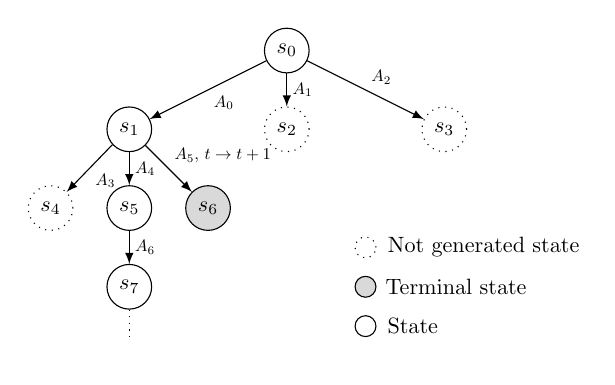
\begin{tikzpicture}[node distance = 1cm]
	\tikzstyle{node}=[circle,align=center,scale=0.8,draw]
	\tikzstyle{nodenotgen}=[circle,dotted,align=center,scale=0.8,draw]
	\tikzstyle{nodeterm}=[circle,fill=gray!30,align=center,scale=0.8,draw]
	\tikzstyle{link}=[->,thin,>=latex]
	\node[node] (s0) at (4,4) {$s_0$};

	\node[node] (s1) at (2,3) {$s_1$};
	\node[nodenotgen] (s2) at (4,3) {$s_2$};
	\node[nodenotgen] (s3) at (6,3) {$s_3$};

	\node[nodenotgen] (s4) at (1,2) {$s_4$};
	\node[node] (s5) at (2,2) {$s_5$};
	\node[nodeterm] (s6) at (3,2) {$s_6$};

	\node[node] (s7) at (2,1) {$s_7$};

	\node[auto,scale=0.8] (s8) at (2,0.2) {};

	\draw[link] (s0) to node [auto,scale=0.6] {$A_0$} (s1); 
	\draw[link] (s0) to node [auto,scale=0.6] {$A_1$} (s2);
	\draw[link] (s0) to node [auto,scale=0.6] {$A_2$} (s3);
	\draw[link] (s1) to node [auto,scale=0.6] {$A_3$} (s4);
	\draw[link] (s1) to node [auto,scale=0.6] {$A_4$} (s5);
	\draw[link] (s1) to node [auto,scale=0.6] {$A_5$, $t \rightarrow t+1$} (s6);
	\draw[link] (s5) to node [auto,scale=0.6] {$A_6$} (s7);
	\draw[-,>=latex,dotted] (s7) to (s8);

	%LEGEND
	\node[node] (l1) at (5,0.5) {}; % {$\phantom{s_1}$};
	\node[nodeterm] (l2) at (5,1)  {}; %{$\phantom{s_1}$};
	\node[nodenotgen] (l3) at (5,1.5) {}; %{$\phantom{s_1}$};
	\node[align=left,rectangle,scale=0.8] (l1t) at (5.6,0.5) {State};
	\node[align=left,rectangle,scale=0.8] (l2t) at (6.15,1.0) {Terminal state};
	\node[align=left,rectangle,scale=0.8] (l3t) at (6.5,1.5) {Not generated state};

\end{tikzpicture}
\caption{Example of a tree}
\label{tree}
\end{figure}
\end{framesubsec}

\section{Search}
\begin{framesec}
    \begin{block}{Searching algorithms}
        \begin{itemize}
            \item UCT: Upper Confidence bounds for Trees
            \item ABCD: Alpha-Beta algorithm Considering Duratives Moves 
        \end{itemize}
    \end{block}
\end{framesec}

\subsection{UCT Search}
\begin{framesubsec}
    \begin{block}{Main ideas}
        \begin{itemize}
            \item UnitAction branching method 
            \item LTD2 state evaluation
            \item Move ordering: Attacking before moving 
        \end{itemize}
    \end{block}
\end{framesubsec}

\subsection{ABCD Search}
\begin{framesubsec}
    \begin{block}{Main ideas}
        \begin{itemize}
            \item Random set from the PlayerActionSubset branching method 
            \item LTD2 state evaluation
        \end{itemize}
    \end{block}
\end{framesubsec}

\section{Results \& Conclusion}
\begin{framesec}
\end{framesec}
\end{document}
